\chapter{\label{chap:caract}Caracterização do Problema}

Neste capítulo, é feito um aprofundamento nos aspectos que tangenciam o sistema proposto neste trabalho. Primeiramente, descreve-se o cenário de estudo e o público alvo. Após esta seção, apresenta-se uma fundamentação teórica em aspectos de acessibilidade, ergonomia e usabilidade; acessibilidade para aplicações móveis Android; sistemas de \emph{text-to-speech} para Android (TalkBack); ontologias e IoT. Em seguida, há a análise de produtos similares já existentes.

\section{Cenário de Estudo e Público Alvo}

Segundo \cite{MOURA2006}, "deficiência visual é um termo empregado para referir-se à perda visual que não pode ser corrigida com lentes por prescrição regular". Este termo diz respeito tanto a cegueira total quanto à baixa visão, onde a pessoa, mesmo com o auxílio de utensílios ópticos, é capaz apenas de diferenciar vultos, claridade e objetos a uma pequena distância \cite{TVESCOLA}. Outra definição de baixa visão é apresentar $^1/_3$ da acuidade perfeita ou menos e ter um campo de visão menor do que 30 graus, sendo a acuidade perfeita de 20/20 e o campo de visão de 160 graus na horizontal e de 135 graus na vertical \cite{ERGO2015}. Já o artigo 70, acerca deficiências físicas, define deficiência visual como:
\begin{directcite}
	cegueira, na qual a acuidade visual é igual ou menor que 0,05 no melhor olho, com a melhor correção óptica; a baixa visão, que significa acuidade visual entre 0,3 e 0,05 no melhor olho, com a melhor correção óptica; os casos nos quais a somatória da medida do campo visual em ambos os olhos for igual ou menor que 60°; ou a ocorrência simultânea de quaisquer das condições anteriores"\ \cite{D5296}.
\end{directcite}

35,6 milhões de brasileiros declaram ter algum tipo de deficiência visual, sendo 1,9 milhão composto por gaúchos. Dos 23,9\% de pessoas com deficiência no Brasil, 18,7\% apresentam alguma deficiência visual, o que torna esta a deficiência com maior manifestação no país. No total, este número compõe 78,4\% da população brasileira com deficiência \cite{IBGE2010}.

No decorrer dos últimos anos, as pessoas migraram, cada vez mais, para os centros urbanos. Mais de $^3/_4$ da população brasileira vive em áreas urbana \cite{IBGE2011} e, em relação às pessoas com deficiência, não é diferente, uma vez que 84,4\% deste grupo também são citadinos \cite{IBGE2010}. Além de viver mais em cidades, a sociedade vem desenvolvendo-se socioeconomicamente, e um dos fatores indicativos deste desenvolvimento é o desfrute de dispositivos móveis. Segundo a Pesquisa Nacional por Amostra de Domicílios \cite{PNAD2014}, 136,6 milhões de brasileiros têm aparelho celular para uso pessoal, 49,4 milhões a mais que em 2008. 

Devido a estes fatores, deseja-se desenvolver um sistema que dê mais independência à pessoa com deficiência visual em suas tarefas cotidianas. Tendo em mente cidadãos que se alimentam em bares ou restaurantes, seja por estudar ou trabalhar fora ou simplesmente por lazer, o cenário atual apresenta dificuldades para quem busca realizar suas refeições em ambientes desconhecidos. 

\section{\label{sec:acessibilidade}Acessibilidade, Ergonomia e Usabilidade em Aplicações Móveis}
Este trabalho busca considerar a importância dos celulares, \emph{smartphones} e dispositivos similares na vida da população brasileira. O desenvolvimento de uma aplicação móvel tornaria o acesso a este sistema mais trivial para grande parte da sociedade. \cite{WCAG20} define “\emph{mobile}” como um termo genérico para uma ampla variação de dispositivos sem fio e aplicações que são fáceis de carregar e usar num vasto conjunto de cenários, incluindo ao ar livre. Estas categorias de aplicações está cada vez mais presente na vida dos brasileiros, sendo em formato de celulares; \emph{tablets}; dispositivos vestíveis, como óculos e relógios inteligentes; e até os sistemas embutidos em automóveis, poltronas de aviões e eletrodomésticos.

Por apresentarem problemas de acessibilidade diferentes dos computadores de mesa, é necessária uma atenção especial para o desenvolvimento da interface destes dispositivos. \cite{WCAG20} propõem quatro princípios que devem ser analisados ao desenvolver-se uma interface amigável e acessível ao usuário:
\begin{description}
    \item [Perceptível] componentes de interface e informações devem ser apresentadas de modo que sejam perceptíveis pelos usuários; os componentes não podem ser invisíveis a todos os sentidos dos usuários \cite{W3C20}. Este princípio pondera sobre o tamanho da tela, o zoom ou o método de ampliação e o contraste. Fatores como tamanho da fonte ajustável e contraste mínimo entre cores de 7:1 devem ser levados em consideração para tornar a aplicação acessível a pessoas com deficiência visual.
    \item [Operável] componentes da interface e a navegação devem ser operáveis, não requisitando ao usuário interações as quais ele não possa performar \cite{W3C20}. O suporte para teclados físicos; a exibição de botões grandes, afastados uns dos outros e posicionados em áreas de fácil acesso; e o uso de gestos triviais podem ser relevantes para determinados grupos com deficiência.
    \item [Compreensível] informações e operações da interface devem ser compreensíveis, sem conteúdos que vão além do entendimento do usuário \cite{W3C20}. Destaca-se, aqui, a preservação de um leiaute em todas as telas; o agrupamento de elementos que desempenham as mesmas ações; a indicação que determinados componentes são acionáveis; e o uso de rótulos ou instruções que expliquem como o sistema funciona.
    \item [Robusto] o conteúdo deve ser robusto o suficiente para ser acessado por diversas tecnologias e, à medida que essas tecnologias avançarem, o sistema deve acompanhar esta mudança e continuar sendo acessível \cite{W3C20}. Para uma aplicação ser robusta, ela deve prover métodos descomplicados para a entrada de dados, permitindo ao usuário inserir informações de diversas formas: através do teclado, toque e voz; reduzir a quantidade de texto apresentada na tela; além de dar suporte às características da plataforma na qual é desenvolvida.
\end{description}

No trabalho apresentado em \cite{ERGO2015}, os autores compilam em sua obra uma série de princípios específicos para a interação entre usuários e dispositivos móveis, sendo eles:
\begin{itemize}
	\item Adequar as aplicações móveis ao contexto do usuário móvel;
	\item Não tentar replicar a experiência do computador de mesa;
	\item Priorizar o conteúdo;
	\item Manter a consistência interna e externa;
	\item Projetar para as diferentes orientações da tela;
	\item Minimizar a carga de trabalho;
	\item Facilitar a navegação;
	\item Minimizar a entrada de dados;
	\item Cuidar com a rolagem de tela;
	\item Apoiar as distrações e interrupções e
	\item Apoiar a personalização da interface.
\end{itemize}
Estes princípios serão aprofundados ao longo do trabalho, buscando enaltecer a experiência do usuário.

% Falar de interface multimodal

\subsection{Acessibilidade em Aplicações Android}

Segundo o Guia para Desenvolvedores Android \cite{DEVACCESS2016}, usuários que apresentam limitações visuais, físicas ou relacionadas ao envelhecimento terão mais acessibilidade ao usar aplicações Android se os serviços de acessibilidade em seus dispositivos estiverem ativados. Desta forma, estes serviços tornarão as aplicações mais acessíveis, mesmo o desenvolvedor não tendo desenvolvido o código da aplicação com o esse intuito. Entretanto, caso uma pessoa esteja desenvolvendo uma aplicação e deseje otimizar sua acessibilidade, há alguns passos que podem ser seguidos:
\begin{enumerate}
	\item Use o atributo “\texttt{android:contentDescription}”. Desta forma, o desenvolvedor pode adicionar textos descritivos aos controles dispostos na tela, o que é deveras significativo, principalmente quando são apresentados imagens, botões e campos de seleção;
	\item Certifique-se de que todos os campos de inserção ou toque possam ser acessados através de um controle direcional ou através de gestos de navegação;
	\item Certifique-se de que alertas e sons estejam acompanhados de elementos ou notificações visuais, uma vez que nem todo usuário será capaz de ouvir os avisos e
	\item Teste sua aplicação usando os serviços de acessibilidade disponíveis. Ligue o TalkBack\footnote{https://play.google.com/store/apps/details?id=com.google.android.marvin.talkback\&hl=pt-br}, por exemplo, e tente usar o aplicativo com este sistema.
\end{enumerate}

Há outras recomendações apresentadas no guia que auxiliam na acessibilidade da aplicação:
\begin{itemize}
	\item Acessar o Guia de Design Acessível do Android\footnote{https://material.io/guidelines/usability/accessibility.html\#}, o qual provê um conjunto de princípios sobre como a interface pode ser desenvolvida, exibindo um conjunto de bons e maus exemplos de design;
	\item Usar os controles de interface já providos pelo sistema, uma vez que eles, por padrão, dão suporte à acessibilidade;
	\item Evitar o uso de controles que desaparecem após um período de tempo e, caso este comportamento seja realmente necessário, prover uma alternativa para essas funções e
	\item Ao usar campos de textos editáveis, fornecer dicas em campos de texto através da marcação "\texttt{android:hint}"\ em código. Desta forma, os usuários sabem que tipo de informação é esperada naquele campo.
\end{itemize}

\subsection{TalkBack}

Disponível nos dispositivos Android, o TalkBack é um leitor de tela desenvolvido pela Google \cite{TALKB2016}. Através de comentários emitidos por voz, este sistema permite que o usuário navegue pelas aplicações sem precisar olhar para o écran. Algumas das características e funcionalidades do TalkBack foram selecionadas e serão listadas a seguir.
\begin{itemize}
	\item Para navegar pela tela através do toque, o usuário pode arrastar lentamente seu dedo sobre o écran. À medida que seu dedo passa sobre os itens apresentados, o sistema reproduzirá as informações através de comandos de voz. Ao encontrar o item desejado, basta tocar duas vezes na tela para acessá-lo.
	\item O TalkBack é composto com um conjunto de gestos particulares, os quais o usuário deve aprender e tem a capacidade de personalizar. Há diversos gestos, todos utilizando um dedo apenas, sendo cada um a representação de uma ação que será executada pelo dispositivo, como: tocar duas vezes na tela para selecionar um item em foco; deslizar rapidamente para a esquerda e para a direita com o intuito de deslocar-se para trás ou para uma página anterior; deslizar para cima e para a direita para abrir o menu de contexto local\footnote{Menu que contém controles referentes ao item focado. Ao ser aberto, pode apresentar opções de navegação, menu de controle do cursor, menu de links, controles de etiquetas ou a opção de editar o nível de controle de deslize.}; etc.
	\item O sistema apresenta definições preestabelecidas as quais buscam auxiliar na navegação e garantir mais segurança para o usuário. Um exemplo de predefinição é a de não ler a senha em voz alta quando esta for digitada, buscando dar mais privacidade e segurança a quem a está inserindo. Há também recomendações feitas pela Google na seção de acessibilidade de seu site; uma recomendação seria o uso do teclado da Google juntamente com o sistema de TalkBack, proporcionando uma experiência com sincronia entre as aplicações e, assim, mais completa e acessível ao usuário.
\end{itemize}

\section{Ontologia}

Nos últimos anos, tornou-se viável a discussão entre sistemas compostos por múltiplos agentes, os quais baseiam-se em estruturas de representação de conhecimento para desenvolver sua comunicação, sendo essas estruturas desenvolvidas a partir de tecnologias semânticas, o que as torna compreensíveis por máquinas \cite{godert2014}. Uma forma de representação do conhecimento é a ontologia, a qual permite a organização do conhecimento, sendo usada em diversos campos e não apenas na IA \cite{ONTOLOGIAI}.

Uma  ontologia  é  uma  forma  de  especificar  conceitos,  objetos  e  relações  numa área de interesse \cite{WEISS1999}, sendo essa uma especificação formal e explícita de uma conceitualização compartilhada, tendo como propósito o compartilhamento e reutilização de conhecimento \cite{UFG2007}.  Esta abordagem científica da ontologia tem como propósito a estruturação do conhecimento, a qual é necessária para a representação da totalidade de um documento, bem como seus tópicos relevantes e o conteúdo de suas declarações \cite{godert2014}. A Figura \ref{fig:ontologia} mostra um exemplo de ontologia.

\begin{figure}[H]
    \centering
    \caption[Exemplo de Ontologia]{\label{fig:ontologia}Exemplo de ontologia para um pequeno negócio, mostrando classes e suas subclasses, relacionamentos e instâncias (indicadas por uma linha tracejada) (Weiss, 2000 -- traduzida)}
    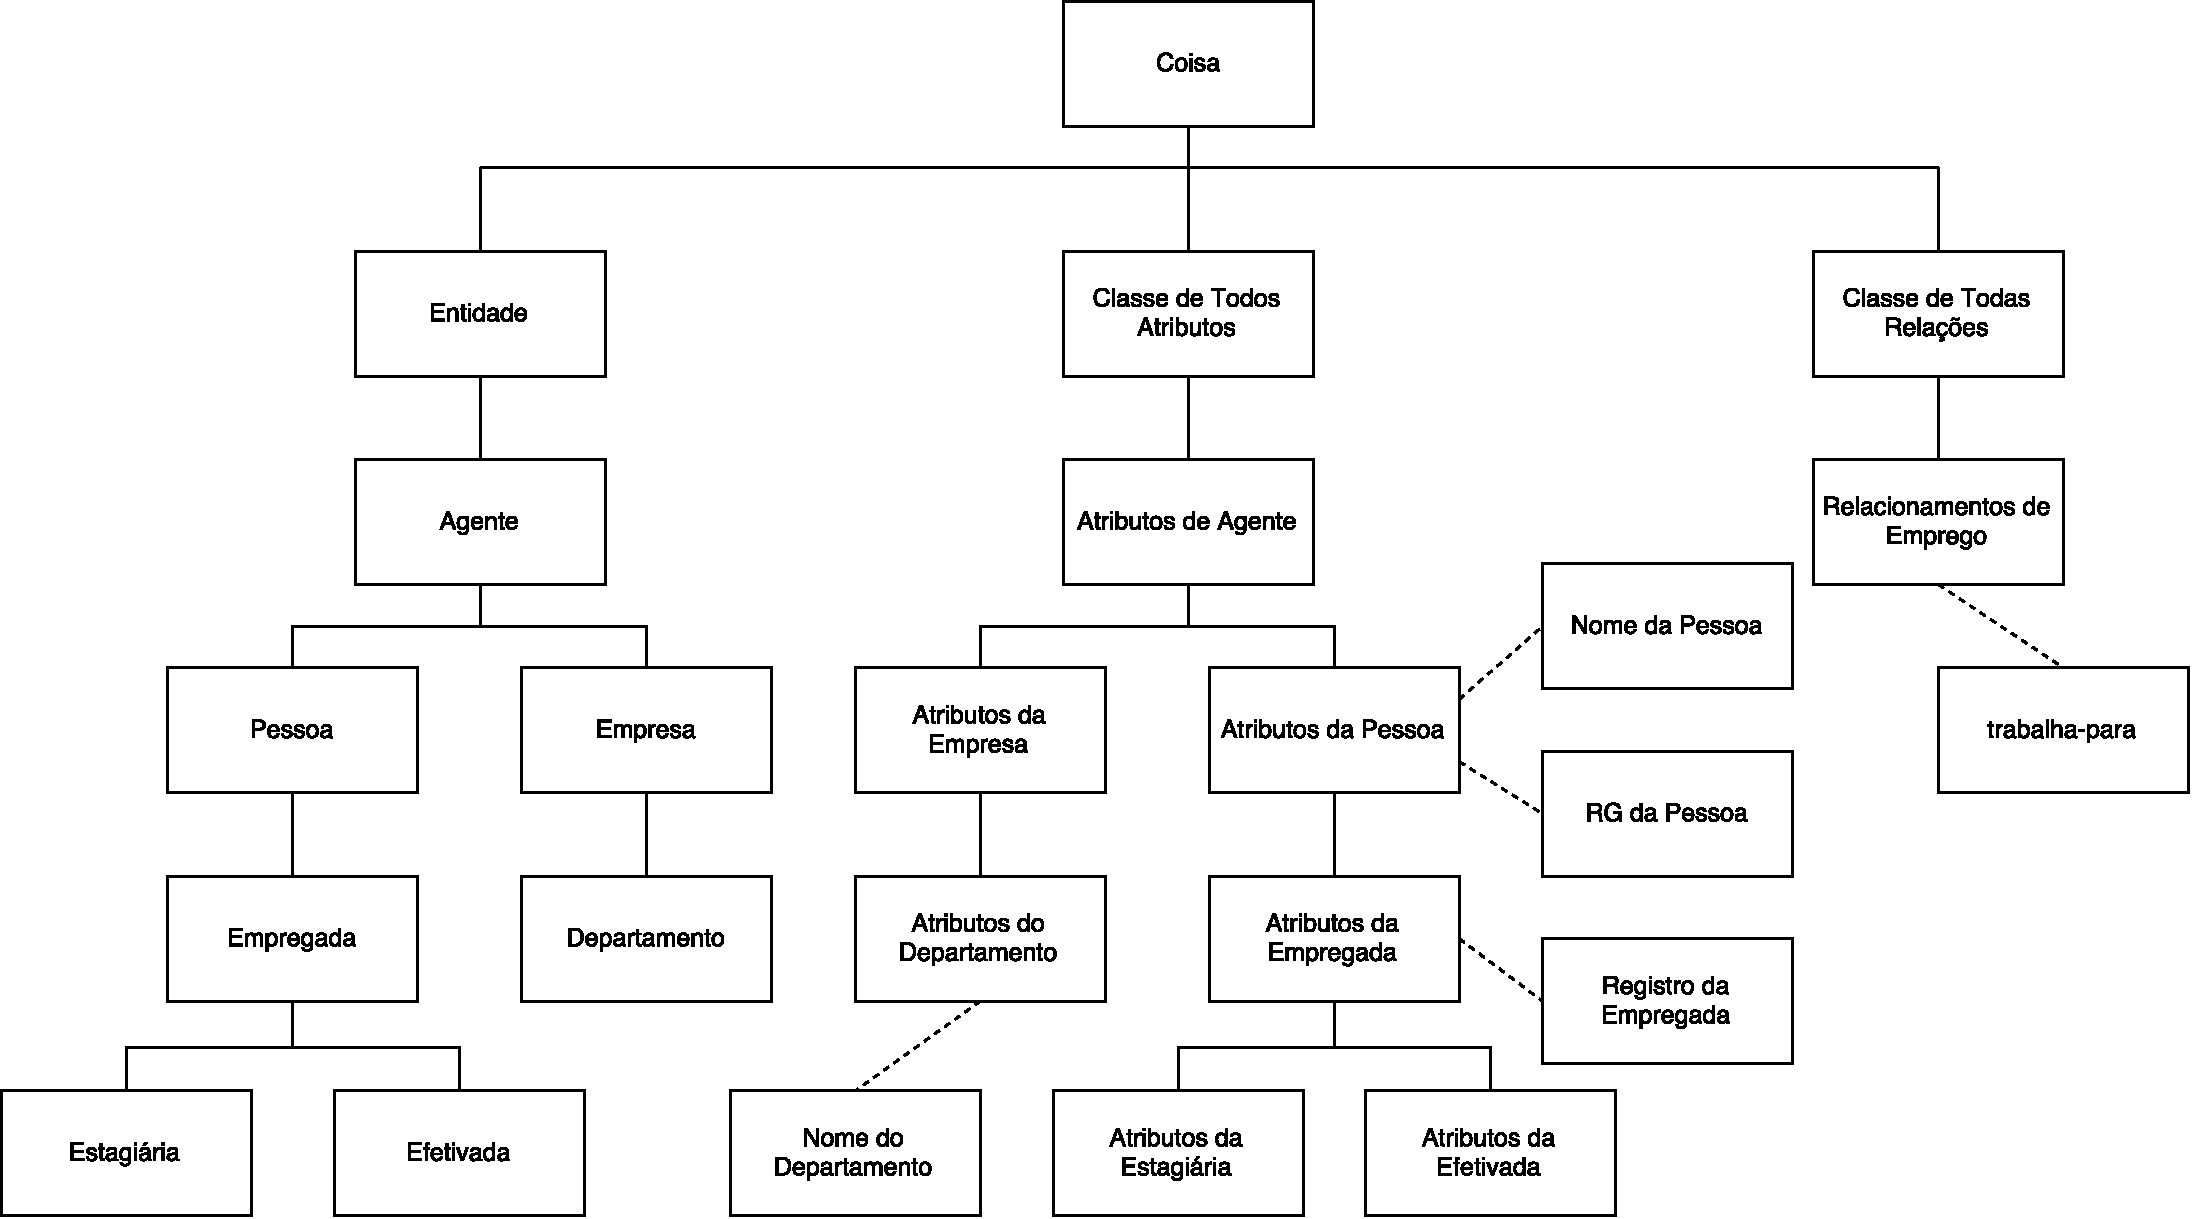
\includegraphics[width=1\textwidth]{pdf/ontology-weiss.pdf}
\end{figure}

Apesar de muito atrelada à área de IA, o uso de ontologias se tornou comum na Internet, possibilitando diversas categorizações em sites de acordo com os conteúdos neles apresentados \cite{NOY2001}. Esta prática facilita a busca de informações realizada por agentes eletrônicos, bem como a integração de gerenciamento do conhecimento e processos comerciais. A partir do uso de ontologias, a estruturação das informações e seu acesso nas redes de computadores tornou-se mais fácil \cite{MAEDCHE2002}.

Uma ontologia não é, simplesmente, uma taxonomia de classes ou tipos: nela, os relacionamentos entre as classes também devem ser descritos, mas suas instâncias não precisam ser representadas.  Ou seja, a ontologia é análoga a um esquema de banco de dados e não ao conteúdo do banco de dados em si (Weiss, 2000). Os conceitos ontológicos podem ser representados através de lógica de primeira ordem (Weiss, 2000), porém também é comum o uso de linguagem natural para a especificação (Morais e Ambrósio, 2007). Um exemplo de especificação de definição em lógica de primeira ordem é dado na Expressão Lógica \ref{el:logica-1-ordem}.

\lstset{
    captionpos=b,
    caption={Exemplo de conceitos representados em lógica de primeira ordem onde a última sentença apresenta uma regra que expressa a noção de um tipo de hierarquia (Weiss, 2000)},
    escapechar=1,
    basicstyle=\ttfamily
}

\vspace{0.4cm}
\begin{lstlisting}[label={el:logica-1-ordem},frame=single]
1$\forall{x}$1 (Bloco x) 1$\Rightarrow$1 (ObjetoFisico x)
(classe Bloco)
(classe ObjetoFisico)
(subclasseDe Bloco ObjetoFisico)
1$\forall{x, y, z}$1 (InstanciaDe x y) 1$\land$1 (SubclasseDe y z) 1$\Rightarrow$1 (InstanciaDe x z)
\end{lstlisting}


Segundo Morais e Ambrósio (2007),  a ontologia,  de acordo com o seu grau de formalismo, será categorizada em uma das quatro categorias abaixo:
\begin{description}
    \item [Altamente informais] são assim categorizadas quando expressas em linguagem natural;
    \item [Semi-informais] também expressas em linguagem natural, entretanto de forma estruturada;
    \item [Semi-formais] ontologias expressas em linguagem artificial definida formalmente;
    \item [Rigorosamente formais] são categorizadas desta forma quando seus termos são definidos a partir de uma semântica formal, teoremas e provas.
\end{description}

Neste trabalho, a ontologia pertence, de acordo com o seu grau de formalismo, à esfera formal. Por outro lado, em relação à sua função, classifica-se no âmbito das ontologias de domínio, isto é, ontologias que: 
\begin{directcite}
    descrevem conceitos e vocabulários relacionados a domínios particulares, tais como medicina ou computação, por exemplo.  Este é o tipo de ontologia mais comum, geralmente construída para representar um “micro-mundo” (Morais e Ambrósio, 2007).
\end{directcite}Esta ontologia será abordada como forma de gestão do conhecimento, todavia, em outros contextos,  sua utilização pode apresentar diversos propósitos,  como o auxílio em processamento de linguagem natural, em web-semântica e na educação em ambientes online (Morais e Ambrósio, 2007).

\subsection{Criando uma Ontologia}
Segundo o guia desenvolvido por \cite{NOY2001}, o primeiro passo a ser seguido é a escolha do domínio e escopo da ontologia. Antes de começar a criá-la, deve-se ter em mente que há diversas ontologias já desenvolvidas, as quais se encontram disponíveis na Internet. Para poupar tempo e retrabalho, uma boa prática é realizar uma pesquisa para descobrir se já não existem trabalhos similares ao que se deseja criar. Sendo assim, é possível aderir bibliotecas de ontologia desenvolvidas para serem reutilizadas, como a DAML Ontology Library\footnote{http://www.daml.org/ontologies/}, e também ter uma ideia de como desenvolver sua própria ontologia.

Para o segundo passo, sugere-se listar os termos considerados importantes neste domínio. Usando como exemplo o tema desenvolvido neste trabalho -- o de um cardápio para restaurantes e estabelecimentos semelhantes --, alguns dos termos que poderiam ser destacados são: \emph{comida} e \emph{bebida}, palavras que representam os tipos de produtos oferecidos no local; \emph{pastel} e \emph{torrada}, para os tipos específicos de lanches; \emph{quantidade}, \emph{ingrediente} e \emph{preço}, para características específicas de cada item do cardápio. A partir desta seleção, torna-se possível a definição das classes e das hierarquias de classes da ontologia que está sendo desenvolvida. Para isso, pode-se começar este desenvolvimento de três formas:
\begin{description}
    \item [De cima para baixo (\emph{top-down})] aqui, define-se os conceitos mais gerais e abrangentes primeiro e, então, os termos mais específicos. Para este trabalho, por exemplo, seria possível começar com termos como \emph{Comida} e, a partir disso, especializar esta classe com subclasses, como \emph{Pastel}, e assim em diante, criando as classes de \emph{Pastel de Carne}, \emph{Pastel de Quatro Queijos}, etc.
    \item [De baixo para cima (\emph{bottom-up})] este processo começa com a definição de termos específicos e, em seguida, com o agrupamento destes termos em classes mais amplas.
    \item [Combinação (\emph{combination})] técnica que consiste na combinação dos dois métodos citados anteriormente. Os termos são definidos sem uma ordem específica e depois são conectados com as classes mais (ou menos) genéricas. Normalmente, é vista como a abordagem mais fácil entre os desenvolvedores de ontologias (Rosch\footnote{Rosch, E., 1978, Principles of Categorization. Em R. E. e B. B. Lloyd, eds. \emph{Cognition and Categorization} pp. 27-48. Lawrence Erlbaum Publishers, Hillside, NJ.} , 1978 citado por \cite{NOY2001}).
\end{description}

A Figura \ref{fig:nivel-ontologia} ilustra os diferentes níveis presentes em uma ontologia:

\begin{figure}[H]
	\centering
	\caption[Níveis da Ontologia]{\label{fig:nivel-ontologia}Diferentes níveis da ontologia de uma lancheria}
    \begin{tikzpicture}
        \node (fig1) at (0,0){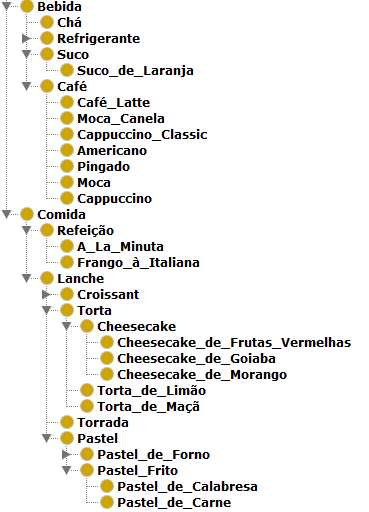
\includegraphics[scale=1]{fig/protege1.png}};
        \node (superior) at (4.5,6.2) {Nível superior};
        \node (intermediario) at (4.5,1.8) {Nível intermediário};
        \node (inferior) at  (4.5,-4.9) {Nível inferior};
        % -------------------------------------- 
        \node (bebida) at (-2,6.6) {}; % superior
        \node (cha) at (-2,6.2) {}; % superior
        \node (refrigerante) at (-0.6,5.8) {}; %superior
        \node (pingado) at (-1,2.3) {}; % intermediario
        \node (moca) at (-1.2,1.9) {}; % intermediario
        \node (cappuccino) at (-0.4,1.5) {}; % intermediario
        \node (cheesecake-morango) at (2.9,-3.4) {}; % inferior
        \node (pastel-calabresa) at (2.2,-5.9) {}; % inferior
        \node (pastel-carne) at (1.8,-6.6) {}; % inferior
        \draw[<-] (bebida) -- (superior);
        \draw[<-] (cha) -- (superior);
        \draw[<-] (refrigerante) -- (superior);
        \draw[<-] (moca) -- (intermediario);
        \draw[<-] (cappuccino) -- (intermediario);
        \draw[<-] (pingado) -- (intermediario);
        \draw[<-] (cheesecake-morango) -- (inferior);
        \draw[<-] (pastel-calabresa) -- (inferior);
        \draw[<-] (pastel-carne) -- (inferior);
    \end{tikzpicture}
\end{figure}

O terceiro passo é o de definição das propriedades das classes, responsável pela descrição de sua estrutura interna. Estas propriedades indicam quais são as características de cada item especificamente, podendo ser propriedades intrínsecas, extrínsecas, partes que compõem esta classe ou a relação desta classe com um outro indivíduo. Subclasses herdam características das classes mais abrangentes; sendo assim, um campo específico deve pertencer à classe mais genérica da hierarquia que possui esta característica, uma vez que suas derivações terão, automaticamente, esta mesma estrutura. No exemplo trabalhado nesta seção, a classe \emph{Bebida} teria informações gerais como \emph{nome}, \emph{temperatura} e \emph{nível de açúcar} e todas suas subclasses herdariam estes campos. As características das classes devem ser tipificadas de acordo com seu valor, podendo ser \emph{Strings}, números, \emph{booleanos}, instâncias, entre outros. No caso de campos caracterizados como instâncias, cria-se uma relação entre a classe que possui o campo (classe \emph{domínio}) e a instância da propriedade (classe de \emph{contradomínio}).

\section{Internet das Coisas}
Com o crescimento maciço de celulares e dispositivos \emph{tablets}, o uso de tecnologias sem fio tornou-se algo comum e fundamental na vida de diversas comunidades \cite{SHIN2014}. Recentemente, múltiplos aparelhos também começaram a se conectar à rede, como veículos, eletrodomésticos, aparelhos vestíveis e até postes de luz, introduzidos com o conceito de \emph{cidades inteligentes} -- cidades com uma infraestrutura monitorada e integrada através da Internet. A União Internacional de Telecomunicações (ITU) define a IoT como uma infraestrutura de rede global dinâmica com capacidades de auto-configuração baseadas em padrões e protocolos de comunicação interoperáveis, onde “coisas” possuem características próprias e estão integradas em uma rede de informações \cite{FRIESS2013}. \cite{FRIESS2013} ressalta que, apesar de recente, a IoT tem sido foco de organizações como Google, Apple e Cisco, outras empresas, como a Huawei, vêm desenvolvendo projetos de cidades inteligentes em grandes cidades brasileiras; um exemplo disso é o \emph{Smart City Innovation Center}, localizado na Pontifícia Universidade Católica do Rio Grande do Sul, em Porto Alegre \cite{RIGON2016}.

\cite{FRIESS2013} destaca a notória intensificação do uso da Internet nos últimos anos. Em 2011, o número de dispositivos conectados à Internet ultrapassou o número de pessoas vivendo no planeta, e a estimativa é que, em 2020, o número de dispositivos esteja entre 26 bilhões e 50 bilhões. A previsão é que megacidades tornem-se inteligentes, entretanto ainda há programas pilotos sendo aplicados para tratar temas como segurança, aceitação por parte dos usuários e validação de ambientes inteligentes cooperativos. Por ser um sistema nupérrimo, \cite{SHIN2014} desenvolveu uma pesquisa buscando entender questões sociais e culturais relacionadas à IoT e concluiu que ainda há uma grande preocupação por parte da sociedade em relação à privacidade.

No momento, a IoT ainda é controversa e exige estudos e experimentos. Todavia, ao ser melhor desenvolvida e implantada em ambientes urbanos, pode ser integrada a diversos sistemas e auxiliar a população em suas tarefas cotidianas. O sistema proposto neste trabalho seria beneficiado através da conexão entre a aplicação móvel e um cardápio inteligente disponível em restaurantes. Este cardápio teria controle do número de instâncias de produtos disponíveis no local e enviaria estas informações à aplicação. Desta forma, seria apresentado ao usuário apenas os alimentos que estão, de fato, sendo vendidos no momento; prática que já é comum em lancherias que disponibilizam seus lanches em uma vitrine.


\section{Trabalhos Relacionados}
Algumas pesquisas foram realizadas com o intuito de conhecer ferramentas e obras similares a esta proposta. A busca foi realizada através de plataformas de pesquisa acadêmica como Google Scholar, ACM Digital Library e IEEE Xplore, além das lojas de aplicativos para Android, a Google Play, e iOS, a App Store; mesmo esta última não sendo o alvo de desenvolvimento desta aplicação, foi considerada importante a análise para conhecer os diversos aplicativos disponíveis no mercado e agregar valor ao trabalho. Foram encontrados alguns projetos que abordam o tema aqui proposto, além de trabalhos que tratam de temas similares. Estes serão apresentados a seguir.

% \subsection{Trabalhos que Tratam de Acessibilidade}

\subsection{\label{subsec:zomato}Zomato}
Desenvolvido para iOS e previamente chamado de Urbanspoon\footnote{https://itunes.apple.com/br/app/urbanspoon-restaurant-food/id284708449?mt=8},  esta aplicação apresenta classificações e críticas sobre restaurantes com o intuito de ajudar o usuário a encontrar a melhor opção para sua refeição. Utilizando dispositivos com, por exemplo, Sistemas de Posicionamento Global (GPS -- \emph{Global Positioning Systems}), o Zomato\footnote{https://itunes.apple.com/br/app/zomato/id434613896?mt=8} detecta restaurantes nas proximidades e apresenta características como avaliações, cardápio e média de preço, permitindo, também, que a pessoa ordene as localidades por proximidade ou popularidade e salve seus locais favoritos. Ao ser realizado um teste com a aplicação, notou-se algumas falhas no seu desenvolvimento. Este não é um aplicativo criado para pessoas com deficiência visual, apenas oferecendo suporte completo para a ferramenta de leitura de tela da Apple, o VoiceOver\footnote{http://www.apple.com/br/accessibility/osx/voiceover/}. Por conta de não ter sido desenvolvido especialmente para usuários com deficiência visual, algumas telas podem apresentar dificuldades ao usuário, como mostrado na Figura ~\ref{fig:zomato1}(b), onde muitos itens acabam sendo sobrepostos.

\begin{figure}[H]
    \centering
    \caption[Ferramenta Zomato]{Telas do aplicativo Zomato}
    \label{fig:zomato1}
    \subfigure[a][Tela inicial da aplicação]
        {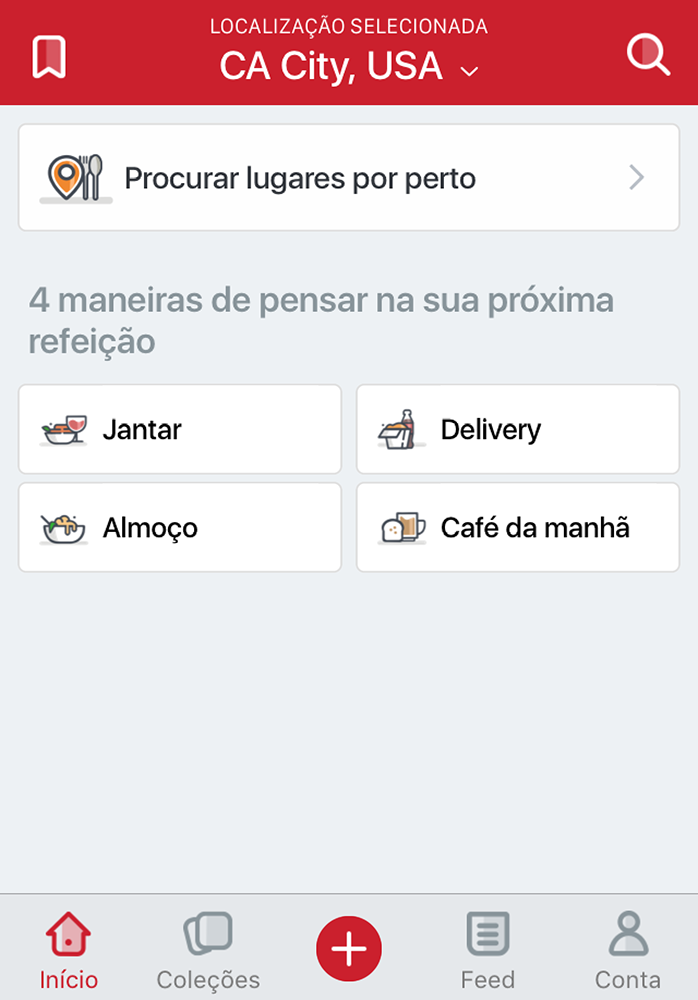
\includegraphics[width=0.27\textwidth]{fig/zomato1.PNG}}
        \qquad
    \subfigure[b][Visualização dos restaurantes no mapa]
        {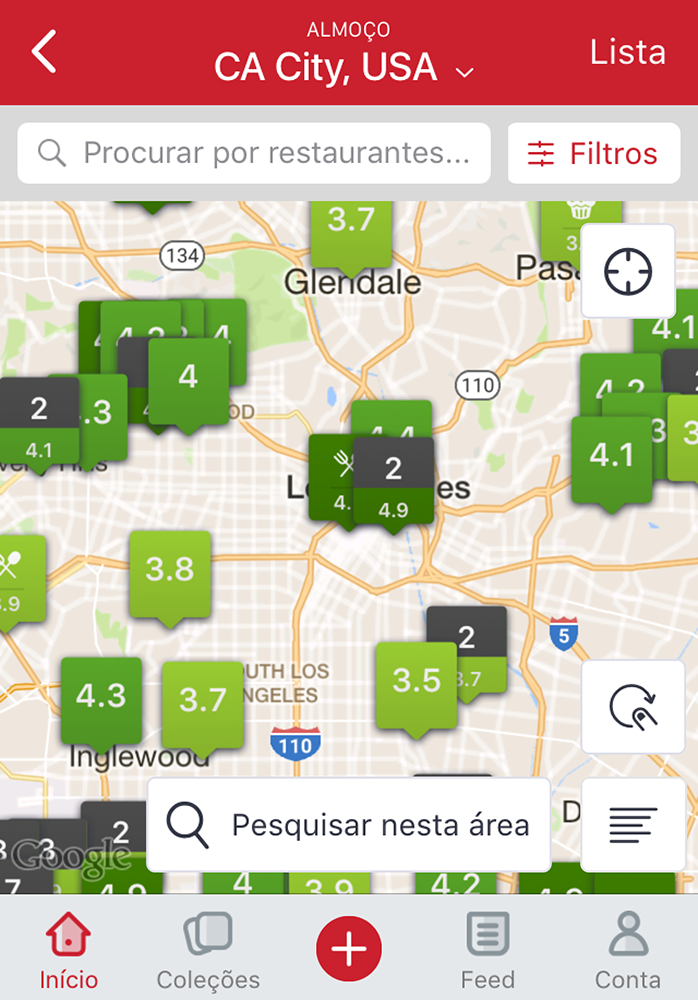
\includegraphics[width=0.27\textwidth]{fig/zomato4.PNG}}
        \qquad
    \subfigure[c][Opção para filtrar resultados]
        {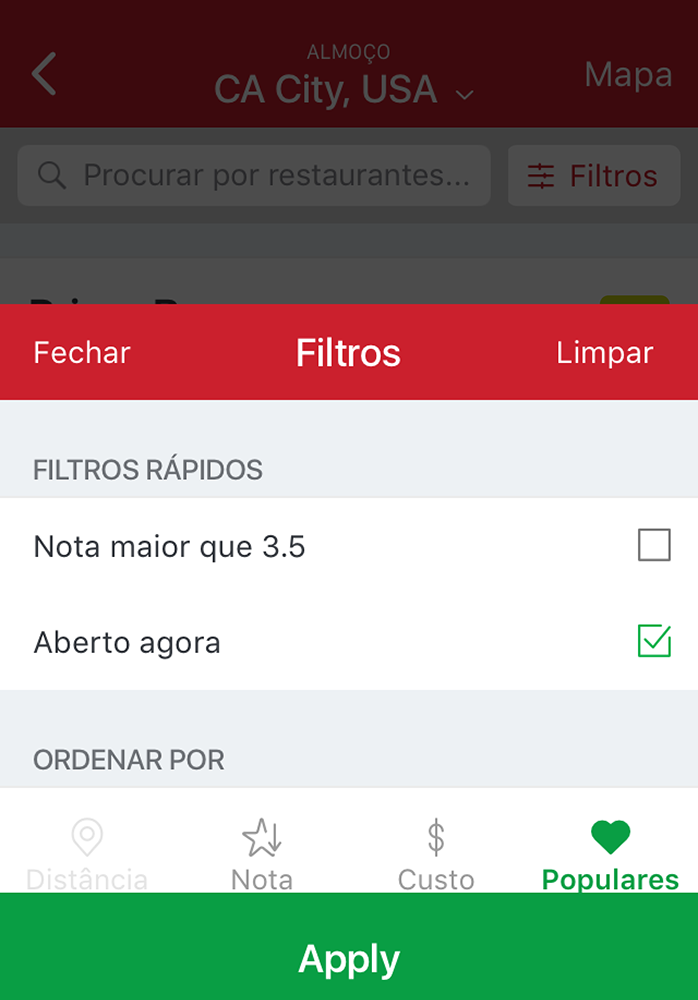
\includegraphics[width=0.27\textwidth]{fig/zomato3.PNG}}
\end{figure}

\subsection{Kapten PLUS}
Um dispositivo de locomoção disponível no mercado é o Kapten PLUS -- Dispositivo de Navegação Pessoal (Figura \ref{fig:fig2}). Através de um GPS, o sistema indica, proferindo comandos, onde o usuário está localizado e quais passos deve seguir para chegar em seu destino. O sistema também é composto por um controle, o qual possui uma interface tátil com botões em alto relevo. Este controle é necessário para que a pessoa possa inserir comandos e navegar pelos menus do sistema. Apesar de compacto, a utilização do sistema pode ser cansativa, uma vez que o usuário deve realizar a inserção de texto através de setas (para cima, para baixo, para esquerda e para direita) e também deve confirmar cada letra ou comando escolhido \cite{KAPTEN}.

\begin{figure}[H]
\centering
\caption[Ferramenta Kapten PLUS]{\label{fig:fig2}Kapten PLUS (Denham, 2011)}
\includegraphics[width=.70\textwidth]{fig/kapten1.jpeg}
\end{figure}

%\subsection{Trabalhos que Conjugam Inteligência Artificial e Acessibilidade a Pessoas com Deficiência Visual}

\subsection{Um Assistente Inteligente para Navegação de Pessoas com Deficiência Visual}
Já no ano de 2001, projetos para o auxílio de pessoas com deficiência visual eram desenvolvidos. Com o intuito de guiar seus usuários pela cidade, o artigo apresenta um sistema que utiliza diversos aparatos anexados ao corpo da pessoa que, juntos, servem como um guia para sua locomoção. Através de um GPS, uma câmera, sinais de áudio e diversos outros artefatos, a aplicação obtém informações sobre o local onde o usuário se encontra e os objetos a sua volta e, com isso, envia-lhe sinais de áudio para que ele possa transitar pela cidade. Esta interação é feita através de um agente incorporado no sistema e é este agente que irá se comunicar com o usuário e indicar-lhe as melhores rotas.

Com a utilização de um agente inteligente, as interações humano-agente se dão através de perguntas feitas pelo usuário que serão respondidas pela máquina, onde as informações fornecidas são calculadas através dos equipamentos embutidos no sistema. A implementação do sistema combina metodologias de IA, como interpretação de imagens, voz, linguagem natural, interpretação de conhecimento e conversação \cite{BOURBAKIS2001}.

\subsection{Um Sistema Robótico para a Localização de Pessoas com Deficiência Visual}
Há locais como aeroportos, centros de conferência e outros ambientes desconhecidos onde cães guias, bengalas e demais equipamentos acabam limitando a pessoa que é cega, não oferecendo o auxílio completo que elas possam necessitar. Em contrapartida, o uso de robôs nestas localidades traz diversas vantagens para o cidadão, uma vez que estes agentes podem traçar caminhos que levem o acompanhante a um ponto desejado, como um portão de embarque ou ao elevador mais próximo.

O agente comunica-se através de comandos reproduzidos em áudio, cuja maioria foi entendida pelos usuários que participaram dos testes. Todavia o reconhecimento dos comandos pela parte do agente não apresentou bons resultados, uma vez que os sistemas de reconhecimento de voz ainda estão em desenvolvimento. Outro problema apresentado pelo sistema é em relação à comunicação entre o usuário e outras pessoas que se encontram no ambiente. Por estar sempre ativo, aguardando comandos, o agente acabava por se confundir ao tentar interpretar o que estava sendo dito \cite{KULYUKIN2002}. 

\subsection{AudioGuider}
AudioGuider -- Sistema Eletrônico para Auxílio em Viagens Baseado em Comandos de Áudio é outra ferramenta que auxilia pessoas com deficiências visuais através do uso de GPS e câmera, com a premissa de ser barato e fácil de carregar. Como outros Sistemas Eletrônicos de Auxílio em Viagens (ETA -- \emph{Electronic Travel Aid Systems}), este dispositivo busca auxiliar os usuários em locais desconhecidos através da captura de imagens e localização do usuário. Além disso, este sistema também faz uso de áudio para indicar a distância entre a pessoa e objetos ou a pessoa e seu destino de chegada, utilizando fatores como volume, frequência e ritmo. Por exemplo: ao indicar um destino, o sistema começa a tocar uma determinada música. No momento em que o usuário estiver a cem metros do local, um som de bipe é emitido e a música começa a diminuir até ele chegar ao seu destino \cite{ZHIGANG2010}.

\subsection{Good Food Talks}
Desenvolvido para auxiliar a população com deficiência visual do Reino Unido, Good Food Talks\footnote{http://goodfoodtalks.com/} é um site que disponibiliza o cardápio de diversos restaurantes de forma acessível, tendo como suporte os aplicativos de acessibilidade do sistemas operacionais iOS\footnote{http://www.apple.com/br/accessibility/ios/voiceover/} e Android\footnote{https://play.google.com/store/apps/details?id=com.google.android.marvin.talkback\&hl=pt\_BR}. Na página inicial, o usuário depara-se com as opções de encontrar restaurantes em sua proximidade ou acessar a lista de restaurantes, além de poder inserir o nome de um restaurante específico. Ao selecionar o local desejado, o cardápio é apresentado na tela, trazendo o nome do item, uma descrição e seu preço. O site também oferece instruções de rota de acordo com a localização da pessoa. Entretanto, para um restaurante se cadastrar no sistema, é necessário pagar uma taxa anual de £199. Além disso, ao acessar a aplicação, foi constatado que, como visto na Figura ~\ref{fig:gft1}(a), a interface nem sempre respeita os princípios citados na seção \ref{sec:acessibilidade}.

\begin{figure}[htb]
    \centering
    \caption[Ferramenta Good Food Talks]{Telas do site Good Food Talks}
    \label{fig:gft1}
    \subfigure[c][Tela inicial da aplicação, onde o menu acaba empurrando o conteúdo principal para baixo]
        {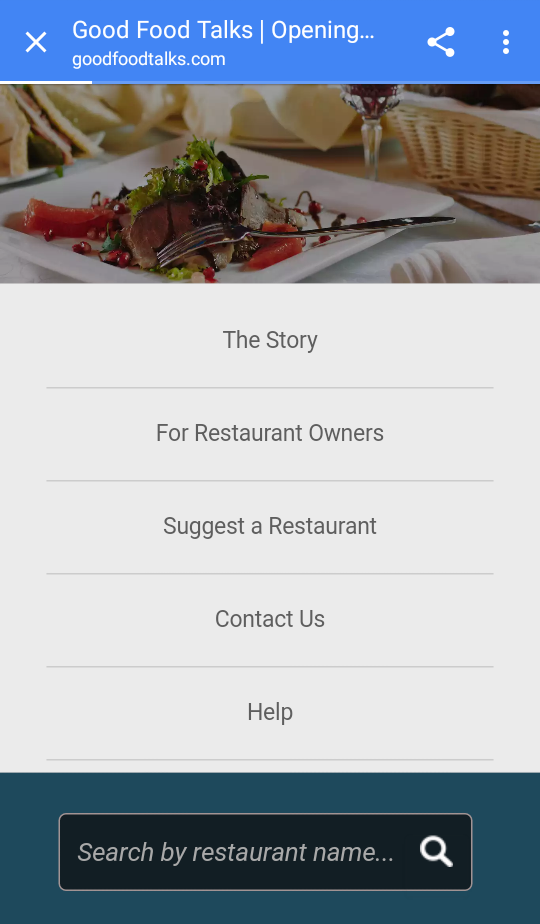
\includegraphics[width=0.27\textwidth]{fig/gft1.png}}
        \qquad
    \subfigure[c][Lista de restaurantes]
        {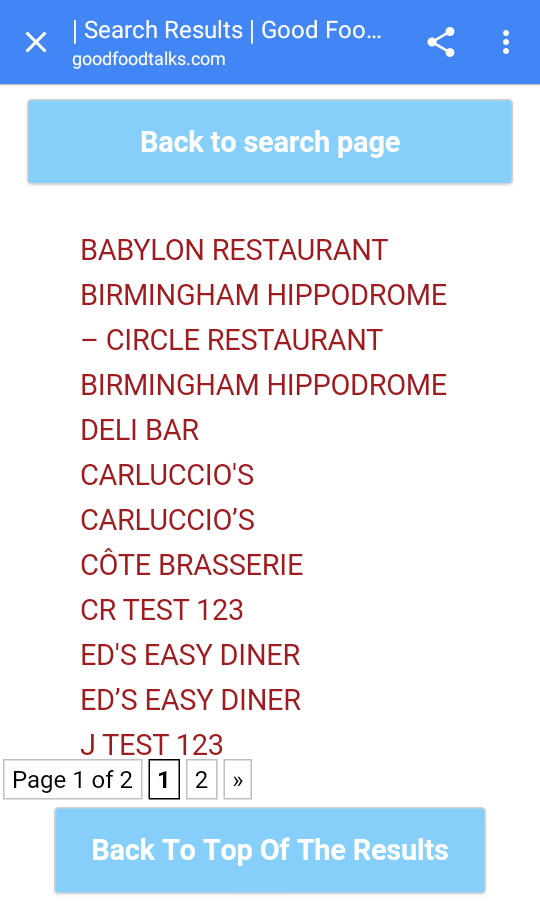
\includegraphics[width=0.27\textwidth]{fig/gft3.png}}
        \qquad
    \subfigure[c][Seção de vinhos do cardápio de um restaurante]
        {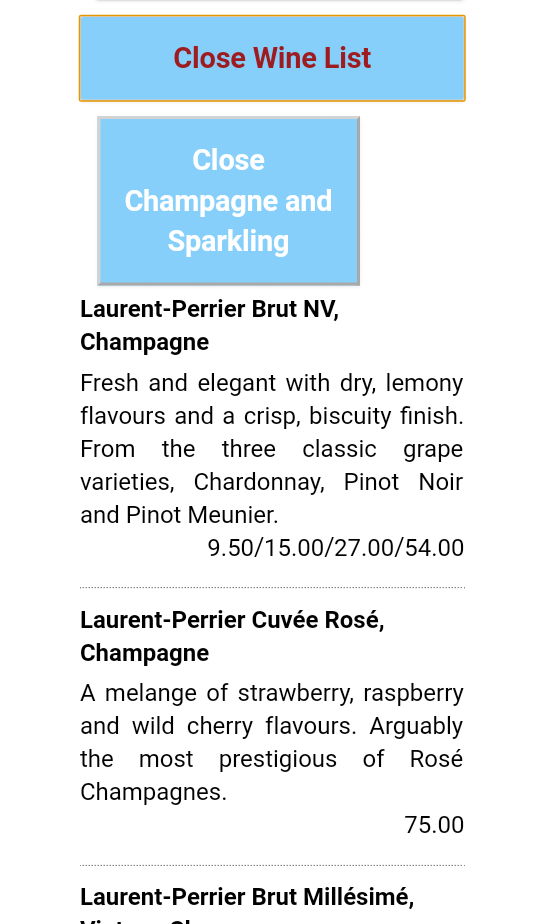
\includegraphics[width=0.27\textwidth]{fig/gft5.png}}
\end{figure}

\subsection{\label{subsec:tappy}Tappy Menu}
Tappy Menu\footnote{https://play.google.com/store/apps/details?id=com.ideal.tappymenu} é um aplicativo criado para dar mais liberdade a pessoas com deficiência visual que buscam acessar menus de restaurantes. De acordo com a descrição do Tappy Menu disponível na Google Play Store\footnote{https://play.google.com/store}, considerou-se necessária a criação desta aplicação, uma vez que as opções de cardápios em braile, fornecidas pelos estabelecimentos, tendem a estar desatualizadas. Ademais, uma parcela de pessoas com deficiência visual não possui domínio sobre a linguagem braile, reforçando a necessidade de tal aplicação. Tappy indica ser uma ferramenta completa para seus usuários, oferecendo cardápios detalhados, com informações nutricionais, ingredientes, preços, entre outros. Todavia, ao instalar e navegar pela aplicação, foi percebida a presença de alimentos que possuem informações parciais (Figura ~\ref{fig:tappy1}(a)) ou informações espalhadas pelas seções do aplicativo (Figuras ~\ref{fig:tappy1}(b) e ~\ref{fig:tappy1}(c)). Desenvolvido nos Estados Unidos, a aplicação dá suporte a onze restaurantes da região.

\begin{figure}[htb]
    \centering
    \caption[Ferramenta Tappy Menu]{Telas do aplicativo Tappy Menu}
    \label{fig:tappy1}
    \subfigure[c][Tela de ingredientes de um dos produtos do cardápio da sorveteria Carvel]
        {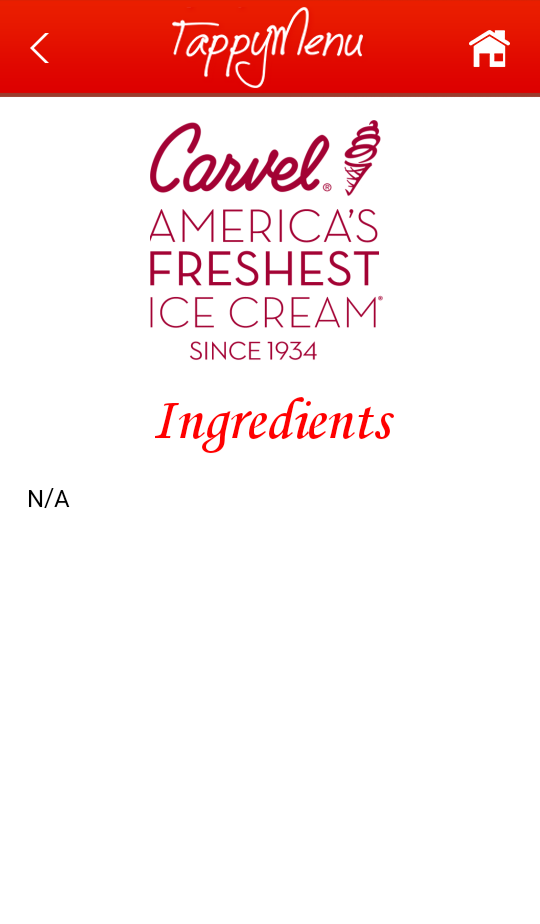
\includegraphics[width=0.27\textwidth]{fig/tappy3.png}}
        \qquad
    \subfigure[c][Descrição das refeições já apresenta os ingredientes para o usuário]
        {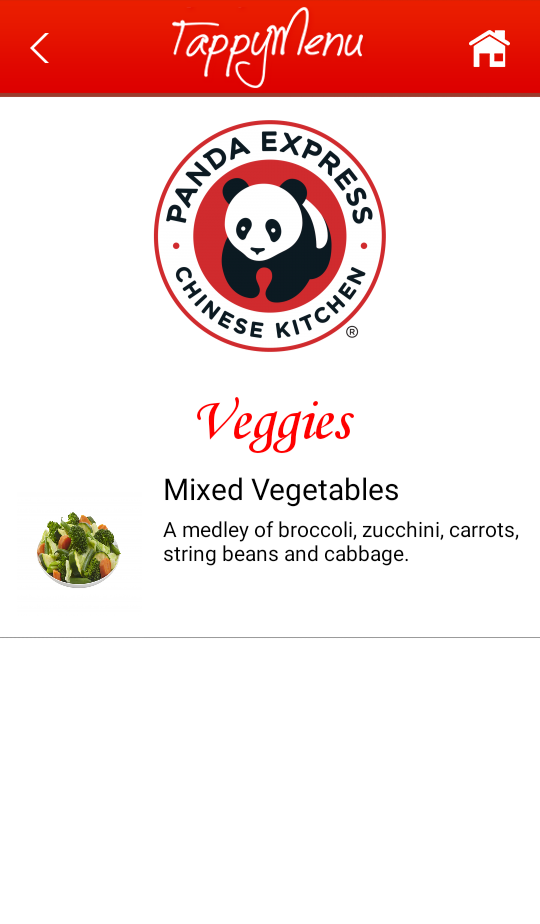
\includegraphics[width=0.27\textwidth]{fig/tappy4.png}}
        \qquad
    \subfigure[c][Tela de ingredientes da opção previamente selecionada, exibindo apenas os ingredientes que causam alergia]
        {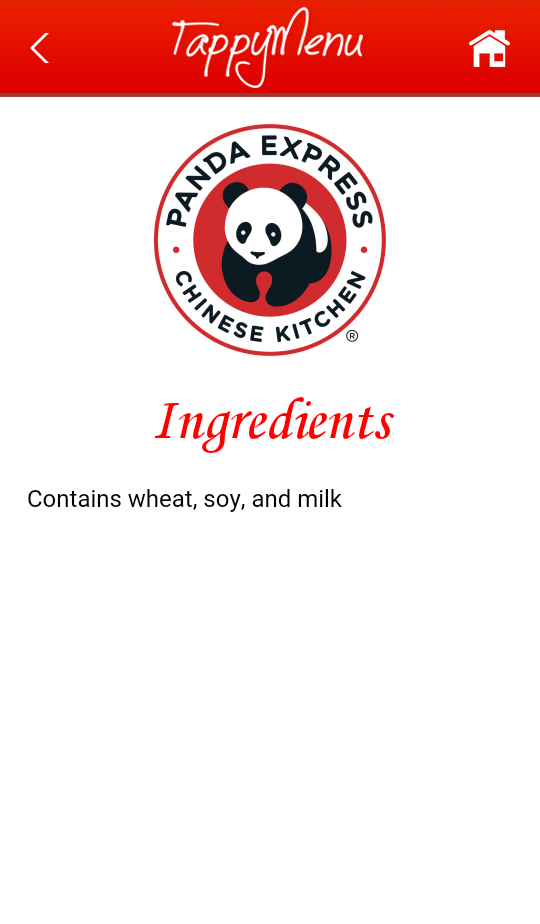
\includegraphics[width=0.27\textwidth]{fig/tappy2.png}}
\end{figure}

\section{Visão Geral das Aplicações}

Os aplicativos para dispositivos móveis testados e apresentados nesta seção (\ref{subsec:zomato} e \ref{subsec:tappy}) apresentaram alguns descuidos ao almejar fornecer uma aplicação acessível e fluída aos seus usuários. Ao serem testadas com as ferramentas VoiceOver e TalkBack (respectivamente), evidenciou-se que algumas melhorias ainda precisavam ser feitas. Além disso, o fluxo da aplicação Tappy Menu não está concisa e pode confundir o usuário. Os demais sistemas não puderam ser testados com ferramentas similares pela restrição de acesso ou falta de softwares que exercem tal função, entretanto a familiarização com os projetos puderam trazer um conhecimento básico sobre o que eles fornecem e como lidam com questões voltadas à acessibilidade. Sendo assim, através da análise feita com este conjunto de aplicações, observou-se artifícios e ideias que podem ser agregadas ao cardápio virtual, bem como práticas que deverão ser evitadas.